% AAAI-Style Two-Column Format (Custom Implementation)
% This uses standard packages to achieve AAAI-like formatting

\documentclass[letterpaper]{article}

% AAAI-like formatting
\usepackage[margin=1.75cm, top=2cm, bottom=2cm]{geometry}
\usepackage{times}
\usepackage{helvet}
\usepackage{courier}
\usepackage[hyphens]{url}
\usepackage{graphicx}
\urlstyle{rm}
\def\UrlFont{\rm}
\usepackage{natbib}
\usepackage{caption}
\frenchspacing
\setlength{\pdfpagewidth}{8.5in}
\setlength{\pdfpageheight}{11in}

% Two-column layout
\usepackage{multicol}
\setlength{\columnsep}{0.5cm}

% Additional packages
\usepackage{amsmath,amssymb,amsfonts}
\usepackage{booktabs}
\usepackage{multirow}
\usepackage{tikz}
\usetikzlibrary{shapes,arrows,positioning,fit,calc}
\usepackage{hyperref}

% Title formatting (AAAI-like)
\makeatletter
\renewcommand{\maketitle}{%
  \begin{center}
    {\Large\bfseries \@title \par}
    \vspace{1em}
    {\normalsize \@author \par}
    \vspace{1.5em}
  \end{center}
}
\makeatother

% Section formatting
\usepackage{titlesec}
\titleformat{\section}{\normalfont\bfseries}{\thesection}{1em}{}
\titleformat{\subsection}{\normalfont\bfseries}{\thesubsection}{1em}{}
\titleformat{\subsubsection}{\normalfont\itshape}{\thesubsubsection}{1em}{}

\setcounter{secnumdepth}{2}

\title{Partisan Discourse on X: An Analysis of Political Polarization in Social Media}

\author{
Ziv Barretto, Agriya Yadav, Kyra Chhetri, Anirban Sen\\
Ashoka University
}

\begin{document}

\maketitle

\begin{multicols}{2}

\begin{abstract}
This paper investigates partisan discourse on X (formerly Twitter), examining how political identities and affiliations shape online communication patterns. We analyze a large-scale dataset of tweets retweeted by Indian politicians from 2020-2023 to understand political polarization in social media. Our methodology combines influencer polarity scoring based on retweet behavior, automated keyword extraction using KeyBERT, and stance classification using a LoRA-adapted large language model. We identify politically polar keywords and classify tweet stances toward these topics to reveal patterns in how ruling and opposition parties engage with different political narratives.
\end{abstract}

\section{Introduction}

The rise of social media platforms has fundamentally transformed political communication and discourse. X (formerly known as Twitter) has emerged as a critical platform for political discussion, serving as a space where politicians, journalists, activists, and citizens engage in real-time conversations about political issues. However, this democratization of political discourse has coincided with growing concerns about political polarization and the formation of ideological echo chambers.

This paper investigates partisan discourse on X, examining how political identities and affiliations shape online communication patterns. We focus on the Indian political context, analyzing how politicians from ruling and opposition parties engage with content from various influencers and how this engagement reflects broader patterns of political polarization.

\section{Literature Review}

% TODO: Add literature review content

\section{Data Collection}

\subsection{Data Source}

We utilize a dataset of tweets provided by Professor Joyojeet Pal, comprising retweets made by Indian politicians on X (Twitter) during the period 2020--2023. The dataset captures the retweet behavior of politicians, allowing us to analyze which external accounts (influencers) are amplified by politicians of different political affiliations.

Each record in the dataset represents a retweet action, containing the original tweet content, the retweeting politician's Twitter handle and party affiliation, and the original author (influencer) of the content.

\subsection{Dataset Statistics}

Table~\ref{tab:dataset_stats} presents the key statistics of our dataset after preprocessing and keyword extraction.

\begin{table}[h]
\centering
\caption{Dataset Statistics}
\label{tab:dataset_stats}
\small
\begin{tabular}{lr}
\toprule
\textbf{Metric} & \textbf{Value} \\
\midrule
Total tweet-keyword pairs & 8,346,024 \\
Unique keywords & 96,528 \\
Unique influencers & 921 \\
Unique retweeting politicians & 16,224 \\
Temporal range & 2020--2023 \\
\bottomrule
\end{tabular}
\end{table}

The temporal distribution of tweets, shown in Table~\ref{tab:temporal_dist}, indicates that 2021 saw the highest volume of retweet activity (41.3\%), followed by 2022 (26.2\%) and 2020 (22.4\%).

\begin{table}[h]
\centering
\caption{Temporal Distribution of Tweets}
\label{tab:temporal_dist}
\small
\begin{tabular}{lrr}
\toprule
\textbf{Year} & \textbf{Count} & \textbf{Percentage} \\
\midrule
2020 & 1,865,448 & 22.4\% \\
2021 & 3,443,611 & 41.3\% \\
2022 & 2,190,794 & 26.2\% \\
2023 & 845,986 & 10.1\% \\
\bottomrule
\end{tabular}
\end{table}

\subsection{Data Structure}

Table~\ref{tab:columns} describes the key columns in our processed dataset.

\begin{table}[h]
\centering
\caption{Dataset Column Descriptions}
\label{tab:columns}
\footnotesize
\begin{tabular}{p{2cm}p{4.5cm}}
\toprule
\textbf{Column} & \textbf{Description} \\
\midrule
\texttt{timestamp} & Date and time of the tweet \\
\texttt{tweet} & Full text content \\
\texttt{retweet\_author} & Retweeting politician handle \\
\texttt{original\_author} & Influencer handle \\
\texttt{retweet\_party} & Political party \\
\texttt{side} & Political bloc (ruling/opp.) \\
\texttt{polarity\_avg} & Influencer polarity score \\
\texttt{tweet\_label} & Inferred political leaning \\
\texttt{keyword} & Extracted topic/keyword \\
\bottomrule
\end{tabular}
\end{table}

\subsection{English Language Filtering}

The original dataset contains tweets in multiple languages, including Hindi and regional Indian languages. For the English analysis pipeline, we filter tweets using an ASCII-ratio heuristic: a tweet is classified as English if at least 85\% of its alphabetic characters are ASCII letters. This approach is computationally efficient for large-scale processing while maintaining reasonable accuracy for language detection.

\section{Methodology}

\subsection{Influencer Polarity Calculation}

A key insight of our approach is that politicians' retweet behavior reveals their political alignments. When a politician retweets content from an external account (influencer), it signals endorsement or amplification of that content. By aggregating retweet patterns across many politicians with known party affiliations, we can infer the political leaning of influencers.

\subsubsection{Polarity Score Formulation}

We first map all political parties to two major blocs: \textit{Ruling} (e.g., BJP, NDA coalition partners) and \textit{Opposition} (e.g., INC, TMC, AAP, and other INDIA bloc parties). For each influencer $i$ and year $y$, we calculate a yearly polarity score:

\begin{equation}
P_{i,y} = \frac{R_{i,y} - O_{i,y}}{R_{i,y} + O_{i,y}}
\label{eq:polarity}
\end{equation}

\noindent where $R_{i,y}$ is the count of retweets the influencer received from Ruling bloc politicians in year $y$, and $O_{i,y}$ is the count from Opposition bloc politicians.

The polarity score ranges from $-1$ (exclusively retweeted by Opposition) to $+1$ (exclusively retweeted by Ruling). We then compute an average polarity score across all available years for each influencer:

\begin{equation}
P_{avg,i} = \frac{1}{|Y_i|} \sum_{y \in Y_i} P_{i,y}
\end{equation}

\noindent where $Y_i$ is the set of years in which influencer $i$ was retweeted.

\subsubsection{Classification Thresholds}

Based on the average polarity score, influencers are classified into three categories:

\begin{itemize}
    \item \textbf{Pro-Ruling}: $P_{avg} \geq 0.5$
    \item \textbf{Pro-Opposition}: $P_{avg} \leq -0.5$
    \item \textbf{Neutral}: $-0.5 < P_{avg} < 0.5$
\end{itemize}

This classification is then propagated to all tweets authored by each influencer, labeling tweets based on the political leaning of their author.

\subsubsection{Justification for This Approach}

Alternative approaches to measuring political polarity include:
\begin{itemize}
    \item \textbf{Hashtag-based}: Inferring polarity from hashtag usage. However, hashtags can be appropriated, used sarcastically, or vary in political signal strength.
    \item \textbf{Content-based}: Using sentiment analysis on tweet text. These methods struggle with context, sarcasm, and nuanced political language.
    \item \textbf{Network-based}: Analyzing follower/following relationships. These are more stable but require extensive social graph data.
\end{itemize}

Our retweet-based approach leverages the revealed preferences of politicians---a retweet represents an explicit endorsement action, providing a more reliable signal than passive following or hashtag co-occurrence.

\subsection{Keyword Extraction with KeyBERT}

To identify the topics discussed in partisan discourse, we employ KeyBERT for automated keyword extraction from tweet text.

\subsubsection{KeyBERT Methodology}

KeyBERT uses sentence-level embeddings to identify keywords and phrases that are semantically similar to the document as a whole. The algorithm:

\begin{enumerate}
    \item Encodes the input document using a Sentence-BERT model
    \item Generates candidate keywords/phrases
    \item Encodes each candidate into the same embedding space
    \item Ranks candidates by cosine similarity
    \item Applies Maximal Marginal Relevance (MMR) for diversity
\end{enumerate}

\subsubsection{Configuration}

We use the following configuration:

\begin{itemize}
    \item \textbf{Model}: \texttt{paraphrase-multilingual-MiniLM-L12-v2}
    \item \textbf{N-gram range}: 1--2 (unigrams and bigrams)
    \item \textbf{Top-N}: 3 keywords per tweet
    \item \textbf{Diversity}: 0.7 (MMR parameter)
\end{itemize}

\subsubsection{Preprocessing}

Before keyword extraction, tweets undergo preprocessing: URL removal, mention extraction (@ handles converted to tokens), hashtag segmentation (e.g., \texttt{\#AatmaNirbharBharat} $\rightarrow$ ``aatma nirbhar bharat''), and whitespace normalization.

\subsubsection{Polar Keyword Selection}

After extracting keywords from all tweets, we identify \textit{polar keywords}---topics that are disproportionately discussed by one political side. A keyword is classified as politically polar if more than 70\% of tweets containing that keyword come from one political bloc.

Table~\ref{tab:polar_keywords} presents the 15 polar keywords selected for stance analysis.

\begin{table}[h]
\centering
\caption{Selected Polar Keywords for Stance Analysis}
\label{tab:polar_keywords}
\footnotesize
\begin{tabular}{lp{2cm}}
\toprule
\textbf{Keyword} & \textbf{Dominant Side} \\
\midrule
caa & Pro-Opposition \\
china & Mixed \\
congress & Pro-Ruling \\
farm\_laws & Pro-Opposition \\
farmers\_protests & Pro-Opposition \\
hindu & Pro-Ruling \\
hindutva & Pro-Opposition \\
kashmir & Mixed \\
kashmiri\_pandits & Pro-Ruling \\
modi & Pro-Ruling \\
muslim & Pro-Opposition \\
new\_parliament & Pro-Ruling \\
rahulgandhi & Mixed \\
ram\_mandir & Pro-Ruling \\
shaheen\_bagh & Pro-Opposition \\
\bottomrule
\end{tabular}
\end{table}

\subsection{Stance Classification}

To understand how different political factions discuss polar topics, we develop a stance classification system that determines whether a tweet expresses support, opposition, or neutrality toward a given keyword/entity.

\subsubsection{Problem Formulation}

Given a tweet $t$ and a target entity (keyword) $e$, the stance classification task predicts one of three labels:
\begin{itemize}
    \item \textbf{Favor}: Support for the entity
    \item \textbf{Against}: Opposition to the entity
    \item \textbf{Neutral}: No clear positive/negative stance
\end{itemize}

\subsubsection{Model Architecture}

We employ a large language model (LLM) adapted for stance classification:

\begin{itemize}
    \item \textbf{Base Model}: Mistral-7B-Instruct, a 7-billion parameter instruction-tuned language model
    \item \textbf{Adaptation}: Low-Rank Adaptation (LoRA), which freezes pre-trained weights and injects trainable rank decomposition matrices
\end{itemize}

LoRA enables parameter-efficient fine-tuning by decomposing weight updates into low-rank matrices:

\begin{equation}
W' = W + BA
\end{equation}

\noindent where $W$ is the frozen pre-trained weight matrix, and $B \in \mathbb{R}^{d \times r}$, $A \in \mathbb{R}^{r \times k}$ are trainable low-rank matrices with rank $r \ll \min(d, k)$.

\subsubsection{Few-Shot Learning}

For each of the 15 target keywords, we curate a set of few-shot examples to guide the model. Each keyword-specific JSON file contains approximately 10 labeled examples: 3 ``favor'', 3 ``against'', 3 ``neutral'', and 1 filler.

During inference, the system dynamically retrieves appropriate few-shot examples based on the target keyword. If keyword-specific examples are unavailable, the system falls back to a global set of examples.

\subsubsection{Manual Annotation}

The few-shot examples and test data were manually annotated through:
\begin{enumerate}
    \item Sampling tweets for each keyword
    \item Deduplication to ensure quality
    \item Multi-annotator labeling
    \item Consolidation into per-keyword JSON files
\end{enumerate}

The annotated data was split 85:15 for training and evaluation with stratified sampling.

\subsubsection{Output Format}

The model generates structured JSON output:

\begin{verbatim}
{
  "stance": "favor|against|neutral",
  "reason": "<brief explanation>"
}
\end{verbatim}

\subsection{Hindi Tweet Analysis Pipeline}

For analyzing Hindi-language tweets, we extend the stance classification pipeline:

\subsubsection{Multilingual Model Support}

The Mistral-7B model supports multilingual input, enabling direct processing of Hindi tweets. The few-shot examples for Hindi tweets are constructed with Hindi text while maintaining the same JSON output format.

\subsubsection{Fallback Mechanism}

The pipeline implements hierarchical few-shot example retrieval:
\begin{enumerate}
    \item Attempt to load keyword-specific examples from \texttt{\{prefix\}\_\{keyword\}\_stance.json}
    \item If unavailable, fall back to a global fallback JSON
\end{enumerate}

This ensures robust inference even for keywords without dedicated few-shot examples.

\subsubsection{Multi-GPU Parallel Inference}

For large-scale processing, we implement a parallel inference pipeline that splits the dataset into chunks, distributes across multiple GPUs, processes each chunk independently, and merges results into a final output file.

\begin{figure}[h]
\centering
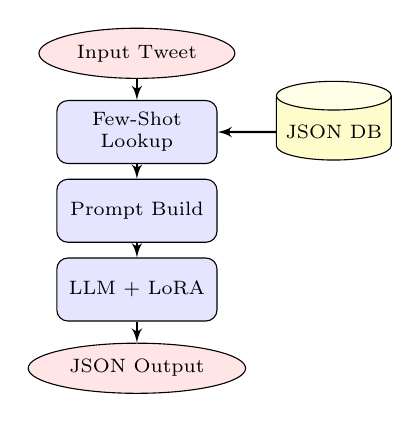
\begin{tikzpicture}[
    node distance=1cm,
    auto,
    block/.style={
        rectangle,
        draw,
        fill=blue!10,
        text width=1.8cm,
        text centered,
        rounded corners,
        minimum height=0.8cm,
        font=\scriptsize
    },
    cloud/.style={
        draw,
        ellipse,
        fill=red!10,
        minimum height=0.6cm,
        font=\scriptsize
    },
    database/.style={
        cylinder,
        cylinder uses custom fill,
        cylinder body fill=yellow!20,
        cylinder end fill=yellow!10,
        shape border rotate=90,
        draw,
        aspect=0.25,
        minimum height=1cm,
        text centered,
        font=\scriptsize
    },
    line/.style={
        draw,
        -latex',
        thick
    }
]

% Nodes
\node [cloud] (input) {Input Tweet};
\node [block, below of=input] (lookup) {Few-Shot Lookup};
\node [database, right of=lookup, node distance=2.5cm] (db) {JSON DB};
\node [block, below of=lookup] (prompt) {Prompt Build};
\node [block, below of=prompt] (llm) {LLM + LoRA};
\node [cloud, below of=llm] (output) {JSON Output};

% Edges
\path [line] (input) -- (lookup);
\path [line] (db) -- (lookup);
\path [line] (lookup) -- (prompt);
\path [line] (prompt) -- (llm);
\path [line] (llm) -- (output);

\end{tikzpicture}
\caption{Stance Detection System Architecture}
\label{fig:architecture}
\end{figure}

\section{Results}

% TODO: Add results content

\subsection{Partisan Network Structure}

\subsection{Content Characteristics}

\subsection{Interaction Patterns}

\subsection{Temporal Dynamics}

\section{Discussion}

% TODO: Add discussion content

\section{Conclusion}

% TODO: Add conclusion content

\section*{Acknowledgment}

We thank Professor Joyojeet Pal for providing the tweet dataset used in this research, and Ashoka University for supporting this work.

\end{multicols}

\end{document}
